In this chapter we discuss the setup of the experiment from start to finish. First we discuss the underlying theory required for the technique. Next, we walk through the walk through the experimental setup, the process of acquiring data and processing it for a single sphere. Finally we address the stretching apparatus, including its calibration process, and analyzing the results. Further details can be found in the appendices.

\section{Measuring Surface Stress via Adhesion}
\subsection{Beyond Hertzian Mechanics and JKR Theory}

Hertzian Mechanics, developed by Heinrich Hertz in the 1800's, allows for the calculation of stress and deformation based on the elastic moduli of the contacted surfaces, as well as their radii of curvature and applied force. While Hertzian mechanics stood for a long time, it neglected to take into account the adhesion energy of the system.  

In 1971, Johnson, Kendall, and Roberts (JKR) sought to remedy this omission by developing a classical theory of contact mechanics that balances the forces of adhesion with elasticity from the bulk and the surface free energy {\cite{johnson1971surface}}. Today, it is still the standard theory used to interpret and soft contact situation. However, it has recently been shown that while JKR theory is a great improvement over Hertztian Mechanics, it breaks down in the elastocapillary regime. \todo[color=green]{add citation} Specifically, at lengths where 
\begin{equation}
\label{EC_regime}
L_{c} \leq \frac{\Upsilon}{E}
\end{equation}
the surface energies compete with those of the bulk and can no longer be ignored. Fittingly, $L_c$ is referred to as the elastocapillary length. By understanding the role of surface tension in soft adhesion, we can measure the physical properties of a balanced system in the elastocapillary regime and hence measure the surface stress and adhesion energy from the balance of forces.



\subsection{Force Balance Derivation}
When materials are soft or small enough, three main forces balance to determine the contact mechanics of the system. Consider a marble sinking into a soft, sticky substrate. Adhesive forces increase the contact area between the marble and the substrate. Increasing the contact area has the effect of ``pulling'' the marble into the gel. As a consequence, the substrate is being compressed [vertically], which is counteracted by the elastic forces within the bulk. This compression also has the effect of stretching the surface of the substrate, which is counteracted by substrate's surface tension. Below, we calculate the energy term associated with each of the forces acting on a dense sphere sinking into a soft substrate. \todo[inline, color=green]{Move to later in chapter: For a silica microsphere, we can ignore the weight of the sphere when calculating the elastic energy term. The force of gravity on the microsphere is negligible compared to the other forces. The density of silica (silicon-dioxide) is $2.65$ g/cm$^3$. For a very large sphere with radius (or is this diameter...) 50 microns, gravity applies a force of roughly 1.02e-08 N.}

\subsubsection{Elastic Energy}
The energy required to make a circular indentation of radius R and depth d can be derived from Hertzian contact mechanics \cite{hertz1882uber, style2013surface,cao2016nanoparticles}. Contact between a sphere and an elastic half space\footnote{i.e. the contact area is $ \ll $ the characteristic radius of the object. A flat plan can be thought of as $ R = \infty $}   is a classic Hertzian contact problem. It is easiest to calculate the force and then integrate to determine the potential energy. For two elastic surfaces in contact with no externally applied forces, the force from elastic contact is:

\begin{equation}
F = \frac{4}{3}E^*R^{1/2}d^{3/2}
\label{elastic_force_eqn}
\end{equation} 
where 
\begin{align*}
\frac{1}{E^*} = \frac{1-\nu_{sphere}^2}{E_{sphere}} + \frac{1-\nu_{substrate}^2}{E_{substrate}} 
\end{align*}
For a glass sphere sinking into a soft substrate, $ E_{sphere} \gg 1-\nu_{sphere}^2 $, so this first term can be dropped as a reasonable approximation\footnote{$\nu_{Si0_2} \approx .17 $ and $ E_{Si0_2} \approx 70 \cross 10^9 $ Pa}. Thus we can approximate $ E^* \approx \frac{E_{substrate}}{1-\nu_{substrate}^2} $. Substituting this into equation (\ref{elastic_force_eqn}), we find:

\begin{equation}
F \approx \frac{4}{3}\frac{ER^{1/2}d^{3/2}}{1-\nu^2}
\label{elastic_force_eqn2}
\end{equation}
Because $F = \frac{\partial U}{\partial d}$, we can simply integrate equation (\ref{elastic_force_eqn2}) to obtain the energy relation:
\begin{equation}
\label{elastic_energy}
U_{elastic} \approx  \frac{ER^{1/2}d^{5/2}}{1-\nu^2}
\end{equation}


\subsubsection{Adhesion Energy}
The energy of adhesion is W multiplied by the surface area in contact (as found above). Namely,
\begin{equation}
\label{W_energy}
U_{adhesion} \approx -2\pi W R d 
\end{equation}
where W is the adhesion energy. \todo[inline,color=yellow]{I think I should explain adhesion somewhere and talk about the Dupre equation 1869. Not sure where I want to put this, however. Maybe some of this stuff and the derivations should actually be in chapter 1. Also ``energy of adhesion = const. * adhesion energy'' lol hmmm}. 



\subsubsection{Surface Energy}
$\Upsilon$ is the surface stress, which is equal to the energy cost per unit area required to create surface via cutting or stretching the material. For a flat substrate being stretched via the indendation of a sphere, the energetic cost is
\begin{equation}
\label{generic_surface_energy}
U_{surface} = \pi \Upsilon_{sv}\Delta A
\end{equation}
where $\Delta A$ is the change in surface area when stretched by part of an indenting sphere (spherical cap). Determining the change in area is a simple geometrical problem.

\begin{equation}
\Delta A = A_{cap} - A_{circle}. 
\end{equation}
Let $ a $ be the base radius of the circle projected on the plane of the substrate's surface. Let R be the radius of the indenting sphere, and d be the depth into which it is stretching. We can find a relationship between these variables using the Pythagorean theorem.

\begin{SCfigure}[][h]
	\begin{minipage}{.5\textwidth}
	\begin{align*}
	&a^2 + (R-d)^2 = R^2 \\
	&a^2 + R^2 - 2Rd +d^2 = R^2 \\
	&a^2 = 2Rd -d^2 \\
	&a^2 + d^2 = 2Rd
	\end{align*}
	\end{minipage}%
	\begin{minipage}{.5\textwidth}
	\centering
	\caption{Spherical Cap Geometry}
	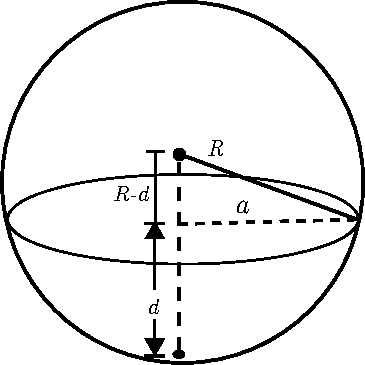
\includegraphics[width=.5\linewidth]{Chapters/Figures/SphericalCap}
	\label{fig:sphericalcap}
	\end{minipage}
\end{SCfigure}
Now, solving for $ \Delta A $ and using the above relationship in the last step, we find:
\begin{align*}
\Delta A &= 2\pi Rd - \pi a^2 \\
&= \pi(a^2+d^2) - \pi a^2 \\
&= \pi d^2
\end{align*}
 Rewriting (\ref{generic_surface_energy}), we can simplify surface energy in this geometry as 
 
 \begin{equation}
 \label{surface_energy}
 U_{surface} = \pi \Upsilon_{sv} d^2
 \end{equation}

\subsubsection{Force Balance}
At static equilibrium, the sum of the energies is:
\[U_{total} = \Upsilon_{sv} \pi d^2 + \frac{cER^{1/2}d^{5/2}}{1-\nu^2} - 2\pi W R d\] 
where c is a geometric factor to be determined in the next step. We can re-arrange the equation such that the sum of forces is equal to zero and differentiate both sides with respect to depth.

\begin{equation*}
\frac{\partial U_{total}}{\partial d} = \Sigma F = 0
\end{equation*}
\begin{equation}
\label{THEeqn}
2 \pi \Upsilon_{sv}d  + \frac{5cER^{1/2}d^{3/2}}{2 \left( 1-\nu ^2 \right) }  - 2 \pi WR = 0
\end{equation}

Where $ c = \frac{8}{5\sqrt{3}} $. This value of c is chosen to recover classical JKR theory, which predicts an indentation of $ d =  \left[\frac{\sqrt{3}\pi W (1 - \mu^2)}{2E} \right]^{2/3}R^{1/3}$ \cite{style2013surface, johnson1971surface}. This energy balance was first published in 2013 by Styles et al. in \textit{Nature Communications} \cite{style2013surface}. \todo[inline, color=green]{Why did you want me to mention Jensen PNAS 2015? Wasn't this the phase separation paper? What connection were you thinking I should make here?}


\subsection{Experimental Approach}
Equation \ref{THEeqn} gives us a quantitative relationship between the spontaneous indentation depth, $ d $, sphere radius, $ R $, and key material properties: $ \Upsilon, E, \nu, \text{and }W $. The Young Modulus, E, and the Poisson ratio, $\nu$ of the substrate can be measured separately for the substrate material. The depth $d$, and the radius $R$ of the sphere can be measured using fluorescent confocal microscopy, as described in section \ref{ch:microscopy}. The only remaining terms, $W$ and $\Upsilon$, the adhesion energy and the surface stress, respectively, can be determined with a two-parameter fit of $ d $ vs. $ R. $ Alternatively, it is possible to measure the adhesion energy separately. This technique, though not critically important to the experiment, is of interest andf exploring if not just for the benefit of adding the capability to the lab.   

Of course, our interest is not just in developing a new technique for measuring, $W$ and $\Upsilon$, but in understanding how those values change when under strain. As needed, we have built our own equibiaxial stretching apparatus capable of maintaining up to 35\% strain in our silicone samples. The design is based off of previous work designed for stretching biological tissues \cite{na2008time} and is similar in design to the apparatus used in the 2017 $\Upsilon(\epsilon)$ measurements \cite{xu2017direct}. Design documents can be found in Appendix A, and an in-depth review of the stretcher can be found in Chapter 3. 

\section{Preparing a Stretchable Substrate}
In the following section, I detail the steps needed in preparation for creating the measurements. My aim is to provide enough details that one could recreate my measurements, forgoing the trouble-shooting process I underwent. 

\subsubsection{Silcone Preparation and Spin Coating} 
In preparing our substrate, there are two important factors to consider: evenness of the surface and thickness. The substrate must be thick enough such that the the indenting microspheres do not feel a significant force from the thin PDMS underlayer. \emph{this probably sounds unclear. Change Later}. We know the stiffness of the gel we are curing, and by having a thick enough coating, we can ensure that the microspheres are only interacting with this gel. 100 $\mu m$ is a reasonable aim, and our substrates generally are between $80-100$ $\mu m$. The second concern is with thickness. In principal, as long as the surface is locally flat with respect to each microsphere, we can determine where the surface level lies and still measure the depth. In reality, it is not difficult to produce an even coating of silicone using a spin-coater. 

Before spin-coating it is useful to coat the underlayer with fluorescent beads. It is not vital, but this is helpful in determining the substrate's thickness. The only information obtained by this coating is the location of the substrate's bottom surface, so a dense bead coverage is not required, and could potentially be harmful if there is light bleeding. I suggest coating the bottom surface with 40nm beads for 1 minute. Full directions for preparing a fluroescent bead solution can be found in Appendix B. After this time, you may return the fluorescent beads back to the solution for re-use. A significant number of beads will remain on the underlayer. To remove some excess, gently wash the substrate with de-ionized water. For a coverslip, simply submerge the entire slip in water and gently remove it at a 45\degree angle, trying to prevent the water from breaking-up into smaller droplets. This process is slightly more difficult for the petri dish due to the larger size. I suggest  (either) using a very large container of water (it can be shallow, really you just need a large opening). If this proves challenging, I have found success using a 1000mL beaker tilted at an angle. It is also possible to use an autopipet for washing; repeat the same process used for the fluorescent bead coating, only use water this time. I have had mixed success with this technique, however. It often leaves a water droplet and has led to an uneven coating of fluorescent beads, manifested as streaks across the surface.

Depending on the silicone, a different amount of time should be waited before spin coating onto the desired surface. We coat our substrate onto glass for "zero applied strain" data or onto PDMS \emph{yeah I gotta look up the brand when I get back. I totally forget.} for stretching data. It is best that the silicone is far enough along in the curing process that it has enough stiffness and cohesiveness to remain on the underlayer when spun. As an extreme example, consider trying to spin-coat water; it would all fling off the underlayer. \emph{is there a better term than underlayer. I'm thinking of the general term for what we use a coverslip or stretchy circle}. For Gelest 9:1, there is no waiting time necessary; Gelest 9:1 cures rapidly. For Dow Corning 1:1, a wait time before spinning of 1 hour was observed. 

To help with the evenness of the coating, it is useful to degas the gel by leaving it in a vacuum chamber for a few minutes. A few small bubbles are not of concern, as the process of transferring the gel to the underlayer is enough to pop any remaining stragglers. I have found that a "glob" of gel roughly half the diameter of the underlayer, with the spin-coater set to 500rpm for 40sec is enough to create an even coating of roughly 100 $\mu m$.  

Coating a coverslip with silicone is a straightfoward process where hardly anything can go wrong. Coating the stretchable PDMS underlayer, however, requires some creativity to find the steps necessary to return the best results. I cut the PDMS disk with an X-acto knife and using a standard Petri \emph{2.5in diameter ...look up} dish as a template. In order to avoid snagging, I suggest cutting out the circle before removing the paper sheets on both sides of the silicone. Taping the Petri dish to the paper is also helpful prevent the dish from slipping while cutting. Unlike the glass coverslip, the PDMS underlayer is not rigid and must be place on a ridgid surface, such as a Petri dish, for spin coating. This leave the possibility that air bubbles could be trapped in between the PDMS and the Petri dish. This is a surefire way to ensure an uneven and frustrating substrate. I suggest removing the top paper sheet of the newly cut PDMS, then placing the Petri dish down upon the exposed silicone. You should now have a Petri dish with a silicone disk on top and a paper sheet on top of that. Using your thumbs, simply do your best to push all the air bubbles from the center outwards. Finally, any tiny air bubbles can hopefully be removed by placing the Petri dish in a vacuum chamber for a few minutes. Now you can coat the PDMS with fluorescent beads and wash as desired before place the petri dish onto the spin-coater and proceeding as described above.

After spin-coating, the silicone requires time to cure. We cure Dow-Corning 1:1 for at room temperature for at least 24 hours. For Gelest 9:1, we oven cure at $70 \degree$ C for at least 24 hours. Either silicone can be cured at room temperature or in the oven so long as a sufficient amount of time is waited, however, we have used this methods to maintain consistency, as well as parallel the techniques used in previous literature \cite{xu2017direct}.

After the silicone cures, it is time to coat the surface with fluorescent beads again. It is important that the beads are dense enough to give a high resolution, yet not so dense as to become indistinguishable; this presents a challenge the MATLAB particle locating software. Secondly, too dense a bead coverage risks light bleeding to vertically adjacent stacks. For the 40nm bead solution prescribed in Appendix B, I suggest letting the solution soak for up to 3 minutes before removing and washing the substrate. While the fluorescent beads chosen are most susceptible to light at \emph{shoot, what wavelength? Like 440?} nm, there is still the risk of photobleaching the fluorophores, and worth dimming the lights in the lab when working with them. 

The final preparation step is to sprinkle silica spheres of a range in size on top of the silicone. This should be done at least 30 minutes before collecting data so that the spheres have time to settle into an equilibrium state into the silicone. From a side view, the final setup should look as follows:



\subsubsection{Fluorescent Confocal Microscopy}
Data was obtained using the Nikon Ti2 Eclipse Microscope as the base, attached to the A2 Confocal \emph{right? The naming has always been confusing}. To take image stacks of the Fluorescent beads, we use a 50x water-immersion objective lens. We set the laser to 440nm and adjust the power (HV) and gain as needed. Generally these values are around 5.0 and 40 respectively. \emph{so, does this mean anything to anyone but me? Like, I don't even know what units that would be, and I doubt it translates to anything other than the Nikon machines, right?} In order to get clear locating, it is important not to saturate the photo-detector. 

\begin{figure}
	\centering
	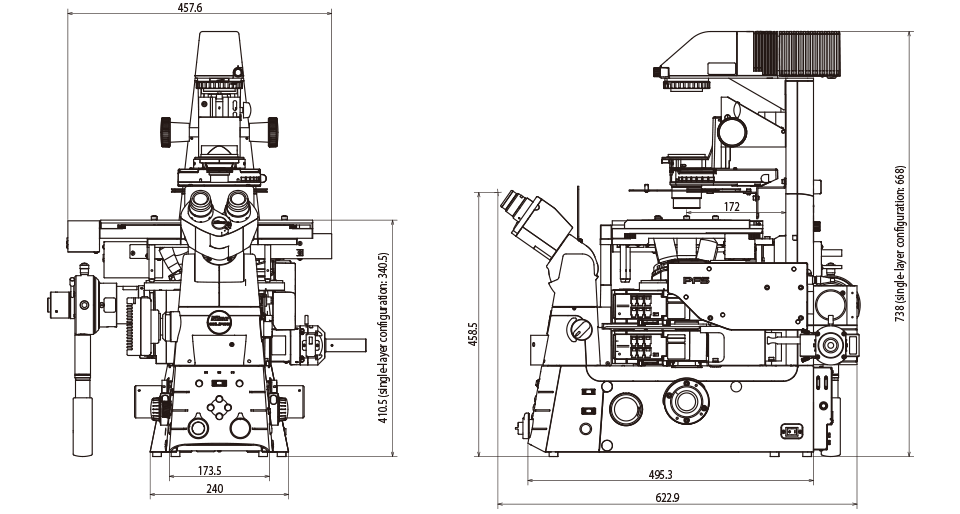
\includegraphics[width=0.7\linewidth]{confocal_stuff/Ti2_diagram_1}
		\caption[Nikon Ti2 Microscope Base]{This may only be here because it's pretty....Also, I'd like to remove the measurements when I have time. Also, not sure how to cite the manual yet.}
	\label{fig:ti2diagram1}
\end{figure}

For silica spheres ranging from $5-50 \mu$m in size, we have found the best scaling factor to be $.104 \mu$m/pixel in the horizontal plane for an image of 1024 x 1024 resolution. We set the vertical step size (z-direction) to $.225 \mu$m/px or $.25 \mu$m/px depending on what the confocal recommended. Both provided adequate vertical resolutions. 16x averaging using the resonant scanner took up to 5 minutes per scan, but provided excellent resolution. 


\section{Stretch Calibration}
% CHAPTER 3


In order to measure the surface stress of soft matter at varying strains, it is necessary to have a device capable of controllably stretching and holding silicone sheets at a constant strain equibiaxially. To achieve this, we built a stretching apparatus based off of the work of Na \cite{na2008time} and Xu \cite{xu2017direct}. Full details of the stretching apparatus can be found in appendix A. 

Aluminum was chosen as the base material because of its sturdy yet malleable nature, making it an excellent material with which to mill. Acrylic was considered, but was not chosen because of its brittle nature; we were concerned about cracking when drilling the UNF threads connecting to the Luer-lock syringe.

Geometrically, the stretching apparatus is constructed of two cylinders connected at the base to create a channel between them. The top of each ring is flat, apart from a slight chamfer to reduce the risk of ripping the sheet needed to be stretched. Each ring is then coated in Dow Corning vacuum grease to make a seal. It is critical that the inner ring has an ample amount of grease so that when a vacuum is pulled in the channel, the sheet will stretch from the center outwards  and not from the edges inwards.  

The stretched sheet is laid over the lubricated apparatus and fixed in place using a 48.7mm diameter by 1.6mm thick rubber O-ring. A removable plastic ring is then placed on top of the o-ring and clamped down using a tension clamp attached to a fitted plastic base. The plastic ring is constructed from an engineering plastic that came from a similar but malfunctioning device used by our colleagues at ETH Zürich. The tension provided by the o-ring and clamp ensure that a solid vacuum is kept and the edges of the sheet are minimally stretched into the trough. The outer ring could easily be laser cut from a plastic or milled out of aluminum if desired. 

To pull a vacuum, a 1/4-28 UNF to female Luer connects the apparatus to a plastic 100ml Luer-lock syringe. We found a more consistent stretch was held by lining the inner walls of the syringe in more Dow Corning vacuum grease. The UNF to female luer connector is stainless steal, and \emph{sealed into place with epoxy resin. Note: I haven't done this yet 190322, but I think I should. But make sure to get the o-ring size first...and i think one size smaller would actually work better}
coated with Dow Corning vacuum grease. The inclusion of a small o-ring between the UNF threads and the cylindrical base proved critical in holding vacuum for sustained periods of time.

The vacuum pull was controlled by a Harvard Apparatus Elite 11 Syringe Pump. Stretching was found to work best at maximum withdrawal rate. Our stretching apparatus has sustained a constant equibiaxial stretch at 36\% strain for as long as 5 hours. Maximum strain percentage and during of maintained stretch is yet to be fully tested.


\section{Calibration}
Originally, we intended to calibrate the strain value induced by the vacuum to the extent that we could predict the induced strain based on the amount of air withdrawn from the stretching apparatus. We withdrew air from the syringe and measured the movement of $~10\mu m$ beads using a 10x air lens on our Nikon confocal microscope. Using the transmission detector allowed us to image the surface of our material with a wide field of view. Strain percentage was calculated using MATLAB code written by Ross (masterGUI then strain Cal). \emph{Note, might come back, cut this and move to next subsubsection. I have it doubled for now.}

There are several obstacles in calibrating the induced strain. First, the stretching apparatus works best when a large strain is applied. Applying small strains one after another works but there is a threshold to induce stretch. No stretching change is visible if less than 2ml is withdrawn from the cylinder per increment. Thus, there is a limited resolution to our calibration data, which would not be a problem if the strain was linear. However, preliminary measurements indicated that the applied strain was nonlinear. This agrees with the with previous results \cite{na2008time} obtained using a similar device. \emph{note to self, double check this is where that graph I'm thinking about actually showed up}. Lastly, the greatest problem with calibrating strain is that we change substrates often. Even if we were to use the same exact sample, by removing it and setting up the device again, there is no way to standardize a zero-applied strain point. To prepare the stretching device, the sample is placed over the opening and a rubber o-ring is placed around the sample to help affix it in place. The sample must then be stretched and wiggled around slightly to remove any snags that could jeopardize the vacuum's efficacy. This means that every time a new sample is prepared, it is in an unknown and unique state of induced strain. It could even have less than zero strain if the sample is loose in large center opening \emph{Think of better name for this.} 

It was thus determined best to measure strain every time we applied a new strain to the silicone substrate and compare it to the substrate's original state. This also assured us that we knew the correct strain value to a higher precision for any given data set. Additionally, with the pleasantly unexpected ability to hold strains exceeding 30\%, the $2\mu$m resolution  limit became superfluous in seeking to measure $\Upsilon(\epsilon)$.


\subsection{Measuring Strain}
Things to talk about here:\\
- Lens and TD settings \checkmark \\
- Tracking code, including the generated images \\
- The tifs including the overlay I used in the APS talk \\

To determine the induced strain, we maximized the field of view. This allows us to see how more more spheres are shifting, and thus gives a more accurate estimate of induced strain. As such, we decided to switch to the bright-field and measure how the spheres were shifting when stretched. We used a 10x air lens in conjunction with the transmission detector on our Nikon Confocal. We adjust the settings to give decent contrast, but it is more important to have the spheres in focus. For our Nikon this usually means setting the Power (HV) to 80. \emph{again...what's HV stand for?} Each sphere reflects light, and it is this reflection that our particle locating software tracks after some image processing. An example image is located below, next to the same image after adjusting the contrast to help our tracking software with particle locating: \emph{um...how well is the image on the right going to print...? Also, the centering is weird for this}

\begin{figure}[h]
	\label{fig:TDpreandpost}
	\begin{tabular}{cc}
		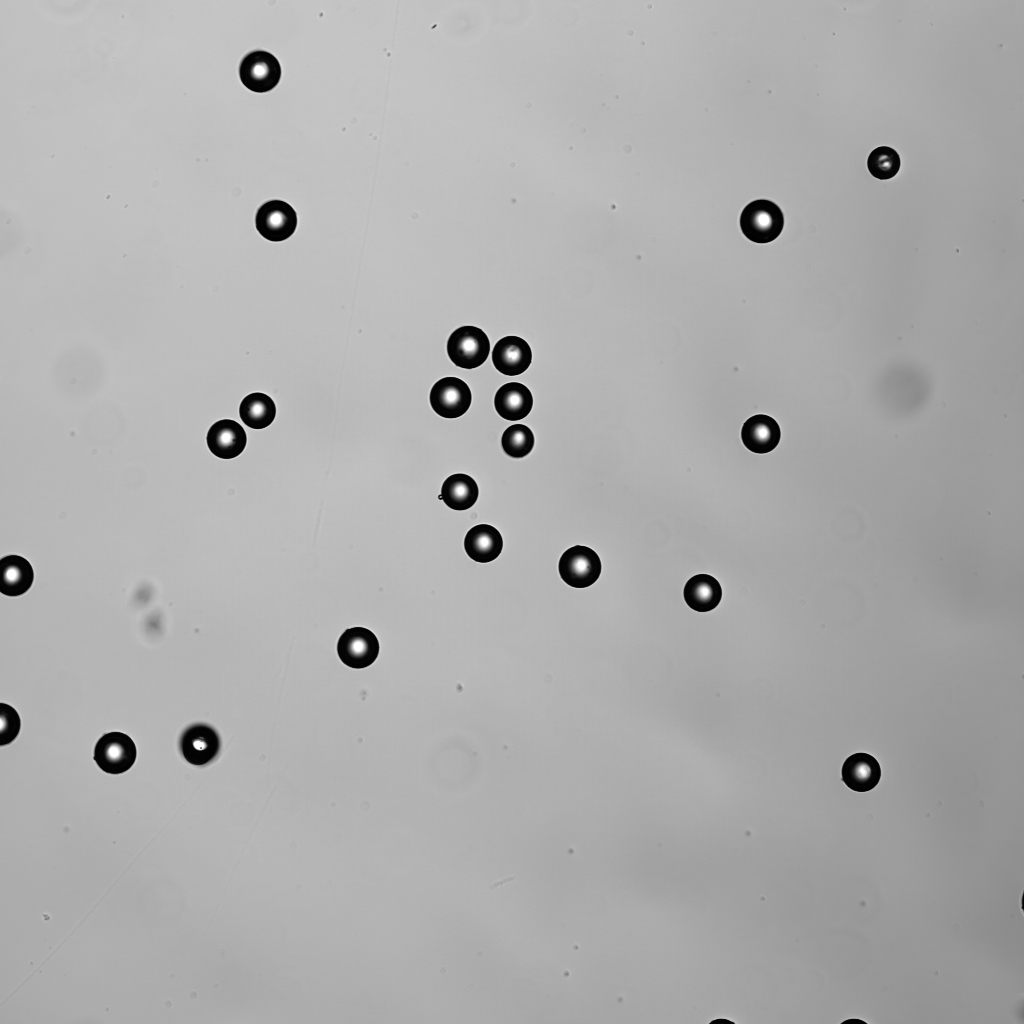
\includegraphics[width= .48\linewidth]{Chapters/Figures/1xzoom_constellation_zeroStrain.png} & 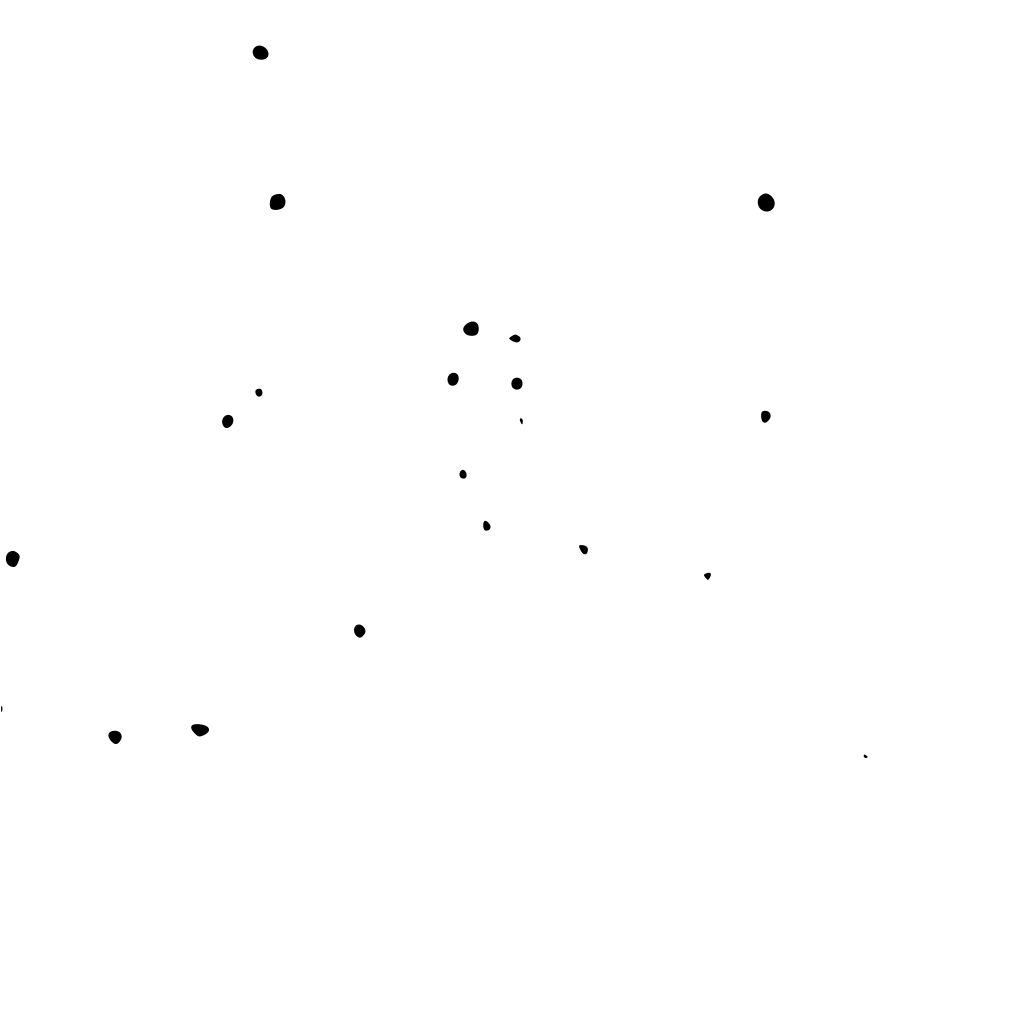
\includegraphics[width= .48\linewidth]{Chapters/Figures/1xzoom_constellation_zeroStrain_supercontrast.png}\\
		Fig. A & Fig. B
	\end{tabular}
	\caption[Bright-field pre and post image processing]{Figure A shows the calibration constellation before any strain is applied. Fig. B shows the same image after processing. Only the sphere reflections remain.}
\end{figure}

To track how the substrate stretches, we first find a centrally located group of spheres, or ``constellation.'' A good constellation is one that easily identifiable for relocation and tracking purposes, and one that has many discrete points in the field of view - i.e. there are plenty of non-overlapping spheres. \emph{It is an added bonus to find 4 spheres perpendicularly located, such that they form the tips of cross.} Though not necessarily, this is useful for a preliminary strain calculation using the built in measuring functions on the Microscope's software. It is nice to track the progression of stretching and ensure the substrate is not preferentially stretching in on direction; this could indicate the substrate is caught in the apparatus. Not only does this ruin the symmetry assumptions being made for our calculation, but it could lead to the substrate tearing if more strain is being applied than expected.

To evacuate the cylinder, we use the the Harvard Apparatus\texttrademark \ Elite Pro Syringe Pump with a 50ml Luerlock syringe. Before beginning any stretching, we withdraw a few ml of air to ensure the substrate is flat and not sagging. At this point we take a picture of the brightfield and call it the ``zero applied strain'' image. We compare all stretched data to this image in order to determine the induced strain. Because of the geometry of the stretching apparatus, along with the way the silicone cures, it is difficult \emph{impossible??} to determine the true strain of the silicone. However, we are most interested in the slope of the $\Upsilon$ vs. $\epsilon$ curve, $\Lambda$, so this is not vitally important.

The induced strain is a tensor of rank two. \emph{If I'm bored and have time, I'd like to add an appendix to talk about this tensor. I think that would be the best way for me to really understand it. That graphic in the book hasn't really stuck with me} Because we are stretching the substrate equally in all directions, we can just look at the magnitude of the tensor and treat the strain as a scalar.     


\begin{figure}[h!]
	\centering
	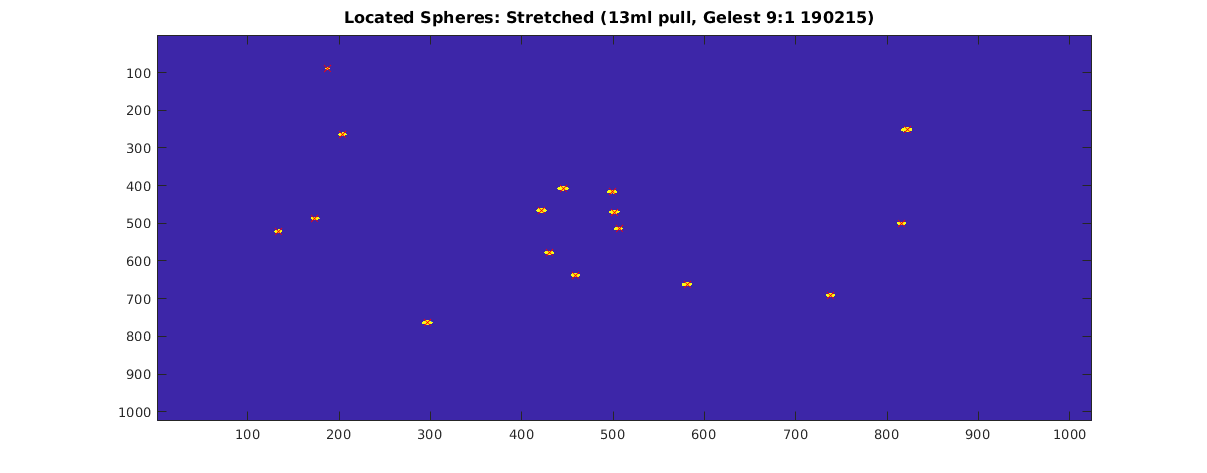
\includegraphics[width=\linewidth]{Chapters/Figures/13ml_stretched_2D_located}
	\caption[Unstretched]{}
	\label{fig:13mlstretched2dlocated}
\end{figure}

\begin{figure}[h!]
	\centering
	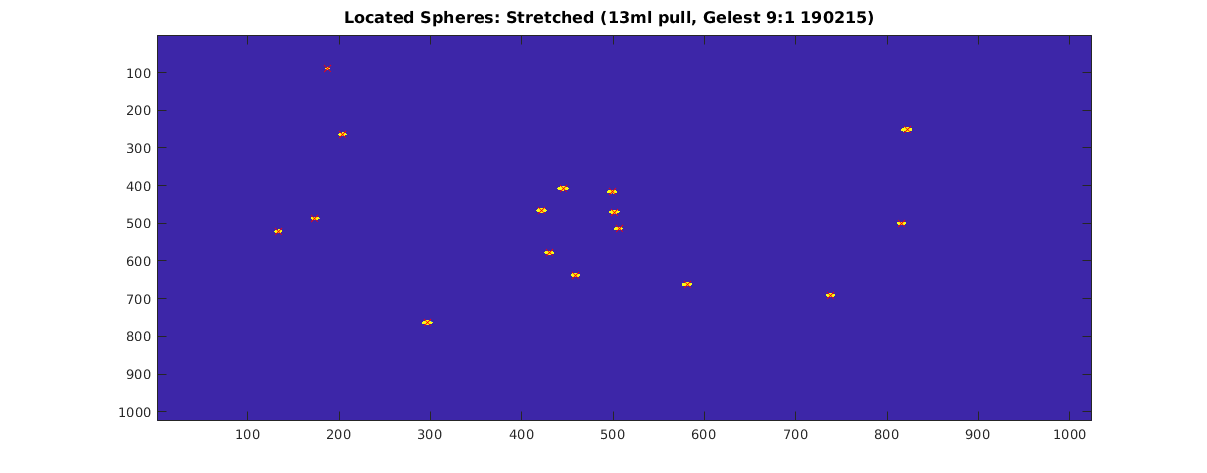
\includegraphics[width=\linewidth]{Chapters/Figures/13ml_stretched_2D_located}
	\caption[Stretched]{These are placeholders for now. I don't really like how they look and I don't think they're totally necessary. It might be nice to keep them if I can clean them up. Especially if I get some nice stretch data with the new DC}
	\label{fig:13mlstretched2dlocated}
\end{figure}

%